\chapter{Introdução} \label{Introducao}
%Contextualizar o problema e motivações
% Motivação (Por quê estes problemas/perguntas são relevantes?)

\section{Endereços e Geocodificação}

\epigraph{Quase tudo que acontece, acontece em algum lugar. Saber o local onde algo acontece pode ser fundamental.}{\cite{longley2013}}

No livro \cite{longley2013} os autores explicam a relação entre a humanidade e a localização. Para eles, é claro que a maior parte da atividade humana é feita no planeta Terra e por isso a vida é fortemente ligada a localidade. Sendo assim, entender e manipular informações geográficas está no cerne de qualquer aplicação que envolve a humanidade. Além disso, os autores explicam que decisões importantes podem causar consequências geográficas. Um exemplo seria uma movimentação financeira, que em um caso mais extremo, poderia causar uma crise econômica em uma determinada região.

No artigo \cite{Zamberg2009}, o autor traz aspectos importantes das informações geográficas que complementam o que foi dito anteriormente. Para ele, endereço é a principal forma de de conceitualizar localização no mundo atual. Isso se deve ao fato dos endereços serem utilizados em diversas aplicações de diferentes campos de estudo, como na saúde \cite{AmericaJournal2001,Kypri2009,Mazumdar2008}, nas ciências sociais \cite{Chow2011}, na análise de criminal ou judiciária \cite{Olligschlaeger1998}, na análise ambiental \cite{Gilboa2006}, na ciência da computação \cite{Zamberg2009}, na economia \cite{Whitsel2006} entre outras.

Para isso, é necessário gerar a representação computacional do endereço, de forma com que as aplicações possam utilizá-lo. A representaçãomais comum segundo \cite{Zamberg2009} é a representação por meio de coordenadas x e y em um plano, geralmente a medida é latitude e longitude. O processo de tranformação em um endereço nessas coordenadas é chamado de Geocodificação ou Georreferenciamento. Para \cite{Zamberg2009} esse processo consiste em 3 etapas:
\begin{itemize}
   \item Processamento do endereço de entrada: o endereço será lido, dividido em componentes (rua, número, bairro, etc), padronizado, cada campo é atribuído a uma categoria e por fim, serão indexadas as categorias necessárias; 
   \item Busca na base referência: de acordo com o algoritmo escolhido, será realizada uma busca na base referência afim de selecionar e classificar potenciais canditados para resposta;
   \item Seleção do(s) canditado(s) para resposta: com a busca realizada será feita uma análise da classificação gerada por ela e serão escolhidos os melhores canditados.
\end{itemize}

Segundo \cite{longley2013}, para além de representar computacionalmente um endereço, o georreferenciamento utilizando latitude e longitude tem diversas vantagens:
\begin{itemize}
   \item Sistema com precisão espacial: é capaz de indicar com precisão alta a localização de um certo endereço;
   \item Permitem cálculos de distância: por ser um sistema espacial, ele permite que a  obtenção da distância e por consequência que outras métricas sejam calculados para o endereço;
   \item Compreensão global: é um sistema utilizado mundialmente, sendo geralmente mais fácil de identificar e compreender; 
\end{itemize}

Apesar de todas as vantagens e aplicações, o processo de geocodificação pode causar informações erradas. No livro \cite{longley2013} os autores nomeiam essas falhas de informação como incertezas. Para coompreender o que é incerteza, é necessário levar em conta outros aspectos da falha na informação. Assim, são incluídos os conceitos:
\begin{itemize}
   \item Erro: Diferença entre o observado e o obtido;
   \item Falta de acurácia: Diferença entre a realidade e a nossa representação da realidade;
   \item Ambiguidade: mais de um valor igual ao outro;
   \item Indefinição: falta de informações necessárias. 
\end{itemize}

Após conceitualizar esses termos, eles definem incerteza como: ``medida da compreensão do usuário sobre a diferença entre o conteúdo de um conjunto de dados e os fenômenos reais que os dados devem representar'' \cite{longley2013}. Ou seja, incerteza é a medida que descreve a compreensão do usuário em relação ao conjunto de dados obtidos e a realidade que esse conjunto de dados pretender observar.  A partir disso, incerteza foi aceita como uma boa medida de avaliação da qualidade dos Sistemas de Informação Geográfica (SIG). 

\begin{figure}[ht]
   \centering
   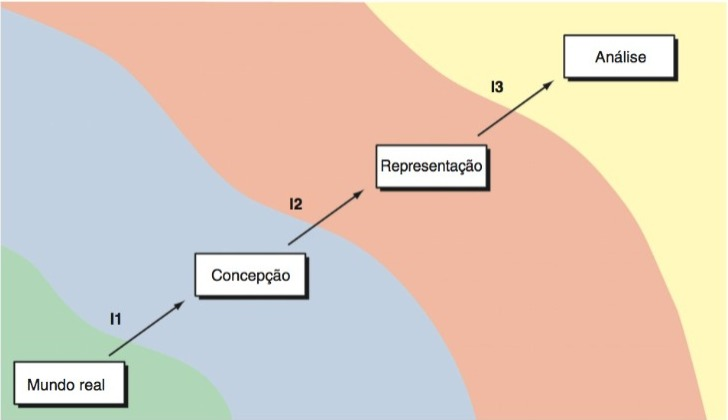
\includegraphics[width=\textwidth]{Figuras/incertezaLivro.jpeg}
   \caption{Retirada do livro \cite{longley2013}. Visão conceitual da incerteza, onde os filtros I1, I2, I3 distorcem a informação original}
   \label{fig:incerteza}
\end{figure}

\section{APIs de Geocodificação e Análise de qualidade}
% Revisão da literatura (O que já foi feito sobre o problema e o que falta fazer?)
Atualmente, no \cite[TerraLAB - Laboratório de pesquisa e capacitação em software]{terralab}, utilizamos de informações geográficas para desenvolvimento das aplicações. Essas aplicações utilizam os endereços geocodificados para desenhar mapas, criar rotas e centros de alcance, denunciar locais, divulgar eventos, etc. Isso indica que a geocodifcação tem muita importância e a qualidade dela traz impactos significativos no que está sendo produzido no laboratório. 
Para obter informações relacionadas a endereços utilizamos a geocodificação obtida a partir das APIs online de geocodifcação. 

Por muitos anos, a principal forma de obter informações geográficas era por meio de um software SIG. Segundo \cite{stein2021geoprocessamento} um Sistema de informação Geográfica (SIG) é um conjunto de ferramentas capaz de analizar e integrar dados geográficos, bem como possibilitar ao usuário acesso facilitado a dados, sem depender de ferramentas como o GPS.
Para \cite{Chow2016}, apesar do SIG ter sido a ferramenta convencional por muitos anos, utiliza-lo para geocodifcação requer um profissional capacitado. A ferramenta demanda o pre-processamento dos dados, criação de um localizador de endereço, customização dos parâmetros, controle de qualidade e correção manual de qualquer falha. Todo esse processo é custoso para o usuário comum. Para ele, a geocodificação utilizando ferramentas online retira do usuário uma grande responsabilidade, a manuteção da base, diminuindo assim os processos para obter a informação e tornando o trabalho menos custoso. 

Apesar de a geocodificação online ser mais simples de utilizar, para que o SIG seja substituído por ela, deve-se considerar sua qualidade em relação a qualidade do SIG. No artigo, \cite{Chow2016} são avaliadas oito ferramentas de gecodificação, sendo duas delas SIGs e o restante, ferramentas da internet. As ferramentas utilizadas foram: SRI ArcGIS Address Locator, CoreLogic PxPoint, Google Maps API,Yahoo!  PlaceFinder,  Microsoft  Bing,  Geocoder.us,  Texas  A and M  University  Geocoder,  and OpenStreetMap (OSM). Para encontrar o erro foi utilizada uma base referência com informações descritivas do endereço (rua, número, cidade, etc) e informações geográficas (latitude e longitude). Essa base é considerada referência pois os dados de latitude e longitude foram obtidos manualmente (GPS ou pesquisa manual). Chamaremos essa e outras bases referência de base padrão ouro. A base em questão possui 940 endereços do estado Texas dos Estados Unidos da America, sendo 78 destes da região de Central Texas, região considerada importante para o autor. Ele então calcula o erro de cada endereço geocodificado como:

\begin{align}
   \epsilon_x &= x_{\text{ref}}, x_{\text{geoc}} \\
   \epsilon_y &= y_{\text{ref}}, y_{\text{geoc}} \\
   \varepsilon_{xy} &= \sqrt{\varepsilon_x^2 + \varepsilon_y^2}
\end{align}
   onde:
   \begin{itemize}
     \item $e_x$ é o erro da longitude,
     \item $e_y$ é o erro da latitude,
     \item $e_xy$ é o erro
   \end{itemize}
   
O estudo mostrou que não há diferença significativa entre as ferramentas online e os SIGs. Tanto os SIGs quanto as ferramentas online tiveram média e desvio padrão do erro similares. Além de taxa de resposta (quantos endereços tiveram resposta para a ferramenta utilizada) de 97,8\% a 100\%, consideradas suficientemente boas. Sendo assim, o estudo teve sucesso ao mostrar que as ferramentas online podem ser utilizadas como substitutivas aos SIGs.
   
Apesar de \cite{Chow2016} ter apresentado resultados significativos, o estudo apresenta limitações. A principal dela é a quantidade dos dados utilizados para fazer essa avaliação e ter focado apenas em uma região (Texas, EUA). O presente trabalho pretende abordar essas limitações ao fazer a análise de outra região do mundo, tendo um enfoque no Brasil, e ampliar a quantidade de dados avaliados. Porém consideraremos apenas ferramentas de geocodificação online (GeoAPIs) por considerar que elas já estão consolidadas no mercado e na acadêmia.  

Outro estudo importante é \cite{Clodoveu2011} que faz uma avaliação da qualidade da geocodificação do Google Maps API fornecida pelo Google Cloud Plataform \cite{GCP}. Nesse estudo, os autores utilizam uma base padrão ouro com os dados de Belo Horizonte, cidade de Minas Gerais, estado do Brasil para essa avaliação. A base conta com mais de 540 mil endereços da cidade e é mantida pela empresa de informática e informação do município de Belo Horizonte - Prodabel \cite{Prodabel}. A empresa atualiza os dados mensalmente
e tem parceria com outras 26 empresas para manter a base o mais correta possível. Ela conta com informações descritivas, sociais e espaciais do endereço. Para medir o erro, foi calculada a distância euclidiana dos pontos geocodificados para os pontos originais. A partir do erro, o estudo faz análises espacias do erro e também relaciona a acurácia descrita pela API com o erro gerado. O estudo mostrou que o Google Maps API tem taxa de acerto de 74,7\%, considerando que acertou se o erro for menor de 150 metros. Outra descoberta foi que o erro é menor nas áreas centrais da cidade, e maior na periferias. Os autores também tentaram fazer uma relação entre erro e renda, porém não foi possível vizualizar nenhuma relação direta. 

Apesar de descobertas importantes, o estudo é limitado na medida que só analisa uma API de geocodificação. Além de analisar apenas uma cidade brasileira, o que impossibilita a generalização dos resultados. O trabalho pretende trabalhar nessas limitações fazendo a análise de uma amostra da mesma base de dados, porém com outras APIs de geodificação. Além disso, iremos fazer uma análise com uma base da região metropolitana de São Paulo. O que traz uma diversidade para nosso estudo. 

\section{Objetivos}
% Objetivo (O que você pretente atingir?)
% Objetivos específicos (objetivos intermediários) 
O principal objetivo deste trabalho é avaliar o erro, a discrepância e a acurácia de cinco APIs utilizadas no laboratório de pesquisa e capacitação em desenvolvimento de software - TerraLAB. As APIs em análise são: Google Maps, TomTom, Open Route Service (ORS), Mapbox e Here. O erro será analisado quanto às respostas fornecidas pelas APIs diferirem do esperado. A discrepância medirá o nível de discordância entre as APIs. Por fim, a acurácia será utilizada para verificar a precisão das respostas fornecidas pelas APIs.

Uma parte essencial do trabalho é compreender os pontos onde essas APIs apresentam falhas, e, portanto, a análise espacial dessas medidas terá grande destaque na pesquisa.

Com isso, gostaríamos de responder as seguintes perguntas:
\begin{itemize}
   \item Qual API das utilizadas erra mais?
   \item Existe algum padrão espacial no erro?
   \item Alguma medida de variância entre as APIs (discrepância) representa o erro? 
\end{itemize}

Para chegar a essas  respostas temos alguns objetivos específicos que devem ser atendidos:
\begin{itemize}
   \item Coletar bases de dados padrão ouro;
   \item Calcular as medidas para avaliação;
   \item Avaliar as distribuição das medidas; 
   \item Correlacionar as medidas; 
   \item Avaliar de que forma o espaço se relaciona com essas medidas.
\end{itemize}





\section{Organização do Trabalho}

Um parágrafo fazendo uma descrição dos capítulos restantes do documento. 

\subsection{Estrutura da Monografia}

Segue uma \textbf{sugestão} para a estrutura da monografia: 

\begin{description}
   \item[Capítulo 1:] Introdução.
   \item[Capítulo \ref{RevisaoBibliografica}:] Revisão Bibliográfica/ Embasamento Teórico (com o referencial teórico e trabalhos relacionados).
   \item[Capítulo \ref{desenvolvimento}:] Metodologia ou Desenvolvimento (material e métodos).
   \item[Capítulo \ref{resultado}:] Resultados e Discussões.
   \item[Capítulo \ref{conclusao}:] Conclusão (e trabalhos futuros).
\end{description}


 









